\chapter{A simple example of chapter title with a large length}
\index{Chapter}

\begin{phrasebox}{}{Fernando Pujaico Rivera}
\label{phrasebox:2}
This box is an environment called \CommandBox{phrasebox} that helped us put phrases. 
In this cases a phrase without title.
\end{phrasebox}


The layout of this book is defined in the \CommandBox{main.tex} 
source file of this book.
\begin{highlightbox}
\begin{verbatim}
%-------------------------------------------------------------------------------
%   Color theme of book
%-------------------------------------------------------------------------------
%%----------------------------------------------------------------------------------------
%   XCOLOR
%----------------------------------------------------------------------------------------
\RequirePackage{xcolor}

%----------------------------------------------------------------------------------------
%   Ways of define colors
%----------------------------------------------------------------------------------------

%% \colorlet{LightRubineRed}{RubineRed!70}
%% \colorlet{Mycolor1}{green!10!orange}
%% \definecolor{light-gray}{gray}{0.95}
%% \definecolor{Mycolor2}{HTML}{00F9DE}
%% \definecolor{orange}{rgb}{1,0.5,0}
%% \definecolor{DarkRed}{RGB}{98,32,6}
%% \definecolor{orange}{cmyk}{0,0.5,1,0}

%----------------------------------------------------------------------------------------
%   INTERNAL, OF THIS FILE, COLOR NAMES -- PALETE OF COLORS 
%
%   Not use this variables in book content
%----------------------------------------------------------------------------------------

% Colores básicos
\definecolor{ColorScheme1}{RGB}{48,48,48}
\definecolor{ColorScheme2}{RGB}{48,48,48}
\definecolor{ColorScheme3}{RGB}{64,64,64}
\definecolor{ColorScheme4}{RGB}{120,120,120}
\definecolor{ColorScheme5}{RGB}{240,240,240}
\definecolor{ColorScheme6}{RGB}{255,255,255}

\DefineBookColorScheme{ColorScheme1}{ColorScheme2}{ColorScheme3}{ColorScheme4}{ColorScheme5}{ColorScheme6}
%----------------------------------------------------------------------------------------
%   All the next color names are OBLIGATORY.
%----------------------------------------------------------------------------------------

% Default
\colorlet{colorDefault}{black} % Define the color used for highlighting throughout the book

% Part-chapter-title
\colorlet{colorTitlePage}{ColorScheme4}
\colorlet{colorPartPageBackground}{ColorScheme4}
\colorlet{colorPartText}{colorDefault}
\colorlet{colorChapter}{colorDefault}
\colorlet{colorSection}{colorDefault}
\colorlet{colorSectionFont}{colorDefault}
\colorlet{colorSubsection}{black}
\colorlet{colorSubsectionFont}{black}

% Boxs
\colorlet{colorAttention}{ColorScheme5}
\colorlet{colorAttentionFrame}{colorDefault}
\colorlet{colorEquationBox}{ColorScheme5}
\colorlet{colorCitationBox}{ColorScheme5}
\colorlet{colorDefinition}{colorDefault}
\colorlet{colorElaboration}{ColorScheme3}
\colorlet{colorElaborationFrame}{colorDefault}
\colorlet{colorExample}{colorDefault}
\colorlet{colorExercise}{colorDefault}
\colorlet{colorPhraseBox}{colorDefault}
\colorlet{colorInformationBox}{colorDefault}
\colorlet{colorLemma}{colorDefault}
\colorlet{colorNotation}{colorDefault}
\colorlet{colorTheorem}{colorDefault}
\colorlet{colorNote}{colorDefault!10}

% Otros
\colorlet{colorLink}{ColorScheme4}
\colorlet{colorIndex}{colorDefault}
\colorlet{colorHeader}{colorDefault}
\colorlet{colorFooter}{colorDefault}

% Init pages
\colorlet{colorPatrocinio}{white}


%----------------------------------------------------------------------------------------
%   COLOR
%----------------------------------------------------------------------------------------
\RequirePackage{color}


%%----------------------------------------------------------------------------------------
%   XCOLOR
%----------------------------------------------------------------------------------------
\RequirePackage{xcolor}

%----------------------------------------------------------------------------------------
%   Ways of define colors
%----------------------------------------------------------------------------------------

%% \colorlet{LightRubineRed}{RubineRed!70}
%% \colorlet{Mycolor1}{green!10!orange}
%% \definecolor{light-gray}{gray}{0.95}
%% \definecolor{Mycolor2}{HTML}{00F9DE}
%% \definecolor{orange}{rgb}{1,0.5,0}
%% \definecolor{DarkRed}{RGB}{98,32,6}
%% \definecolor{orange}{cmyk}{0,0.5,1,0}

%----------------------------------------------------------------------------------------
%   INTERNAL, OF THIS FILE, COLOR NAMES -- PALETE OF COLORS 
%
%   Not use this variables in book content
%----------------------------------------------------------------------------------------

% Color theme
\definecolor{ColorScheme1}{RGB}{16,81,15}
\definecolor{ColorScheme2}{RGB}{217,168,91}
\definecolor{ColorScheme3}{RGB}{255,249,128}
\definecolor{ColorScheme4}{RGB}{105,46,60}
\definecolor{ColorScheme5}{RGB}{182,106,70}
\definecolor{ColorScheme6}{RGB}{240,240,240}

\DefineBookColorScheme{ColorScheme1}{ColorScheme2}{ColorScheme3}{ColorScheme4}{ColorScheme5}{ColorScheme6}
%----------------------------------------------------------------------------------------
%   All the next color names are OBLIGATORY.
%----------------------------------------------------------------------------------------

% Default
\colorlet{colorDefault}{ColorScheme1} % Define the color used for highlighting throughout the book

% Part-chapter-title
\colorlet{colorTitlePage}{ColorScheme4}
\colorlet{colorPartPageBackground}{ColorScheme5!50!black}
\colorlet{colorPartText}{colorDefault}
\colorlet{colorChapter}{colorDefault}
\colorlet{colorSection}{colorDefault}
\colorlet{colorSectionFont}{colorDefault}
\colorlet{colorSubsection}{black}
\colorlet{colorSubsectionFont}{black}

% Boxs
\colorlet{colorAttention}{ColorScheme3}
\colorlet{colorAttentionFrame}{colorDefault}
\colorlet{colorEquationBox}{ColorScheme6}
\colorlet{colorCitationBox}{ColorScheme6}
\colorlet{colorDefinition}{colorDefault}
\colorlet{colorElaboration}{colorDefault}
\colorlet{colorElaborationFrame}{colorDefault}
\colorlet{colorExample}{colorDefault}
\colorlet{colorExercise}{colorDefault}
\colorlet{colorPhraseBox}{colorDefault}
\colorlet{colorInformationBox}{colorDefault}
\colorlet{colorLemma}{colorDefault}
\colorlet{colorNotation}{colorDefault}
\colorlet{colorTheorem}{colorDefault}
\colorlet{colorNote}{colorDefault!10}

% Otros
\colorlet{colorLink}{colorDefault}
\colorlet{colorIndex}{colorDefault}
\colorlet{colorHeader}{colorDefault}
\colorlet{colorFooter}{colorDefault}
\colorlet{colorTableBackground}{colorDefault!10}
\colorlet{colorTableLine}{white}
\colorlet{colorEnumerateBackground}{colorDefault}
\colorlet{colorEnumerateFont}{white}

% Init pages
\colorlet{colorPatrocinio}{ColorScheme6}


%----------------------------------------------------------------------------------------
%   COLOR
%----------------------------------------------------------------------------------------
\RequirePackage{color}


%%----------------------------------------------------------------------------------------
%   XCOLOR
%----------------------------------------------------------------------------------------
\RequirePackage{xcolor}

%----------------------------------------------------------------------------------------
%   Ways of define colors
%----------------------------------------------------------------------------------------

%% \colorlet{LightRubineRed}{RubineRed!70}
%% \colorlet{Mycolor1}{green!10!orange}
%% \definecolor{light-gray}{gray}{0.95}
%% \definecolor{Mycolor2}{HTML}{00F9DE}
%% \definecolor{orange}{rgb}{1,0.5,0}
%% \definecolor{DarkRed}{RGB}{98,32,6}
%% \definecolor{orange}{cmyk}{0,0.5,1,0}

%----------------------------------------------------------------------------------------
%   INTERNAL, OF THIS FILE, COLOR NAMES -- PALETE OF COLORS 
%
%   Not use this variables in book content
%----------------------------------------------------------------------------------------

% Color theme
\definecolor{ColorScheme1}{RGB}{43,79,96}
\definecolor{ColorScheme2}{RGB}{189,199,201}
\definecolor{ColorScheme3}{RGB}{234,211,203}
\definecolor{ColorScheme4}{RGB}{132,84,96}
\definecolor{ColorScheme5}{RGB}{120,120,120}
\definecolor{ColorScheme6}{RGB}{240,240,240}

\DefineBookColorScheme{ColorScheme1}{ColorScheme2}{ColorScheme3}{ColorScheme4}{ColorScheme5}{ColorScheme6}
%----------------------------------------------------------------------------------------
%   All the next color names are OBLIGATORY.
%----------------------------------------------------------------------------------------

% Default
\colorlet{colorDefault}{ColorScheme1} % Define the color used for highlighting throughout the book

% Part-chapter-title
\colorlet{colorTitlePage}{ColorScheme4}
\colorlet{colorPartPageBackground}{ColorScheme5!50!black}
\colorlet{colorPartText}{colorDefault}
\colorlet{colorChapter}{colorDefault}
\colorlet{colorSection}{colorDefault}
\colorlet{colorSectionFont}{colorDefault}
\colorlet{colorSubsection}{black}
\colorlet{colorSubsectionFont}{black}

% Boxs
\colorlet{colorAttention}{ColorScheme3}
\colorlet{colorAttentionFrame}{colorDefault}
\colorlet{colorEquationBox}{ColorScheme2!50}
\colorlet{colorCitationBox}{ColorScheme2!50}
\colorlet{colorDefinition}{ColorScheme4}
\colorlet{colorElaboration}{ColorScheme4}
\colorlet{colorElaborationFrame}{colorDefault}
\colorlet{colorExample}{ColorScheme4}
\colorlet{colorExercise}{ColorScheme4}
\colorlet{colorPhraseBox}{ColorScheme2}
\colorlet{colorInformationBox}{ColorScheme4}
\colorlet{colorLemma}{ColorScheme4}
\colorlet{colorNotation}{ColorScheme4}
\colorlet{colorTheorem}{ColorScheme4}
\colorlet{colorNote}{ColorScheme4!10}

% Otros
\colorlet{colorLink}{ColorScheme4}
\colorlet{colorIndex}{colorDefault}
\colorlet{colorHeader}{colorDefault}
\colorlet{colorFooter}{colorDefault}
\colorlet{colorTableBackground}{colorDefault!10}
\colorlet{colorTableLine}{white}
\colorlet{colorEnumerateBackground}{colorDefault}
\colorlet{colorEnumerateFont}{white}

% Init pages
\colorlet{colorPatrocinio}{ColorScheme2!50}


%----------------------------------------------------------------------------------------
%   COLOR
%----------------------------------------------------------------------------------------
\RequirePackage{color}


%%----------------------------------------------------------------------------------------
%   XCOLOR
%----------------------------------------------------------------------------------------
\RequirePackage{xcolor}

%----------------------------------------------------------------------------------------
%   Ways of define colors
%----------------------------------------------------------------------------------------

%% \colorlet{LightRubineRed}{RubineRed!70}
%% \colorlet{Mycolor1}{green!10!orange}
%% \definecolor{light-gray}{gray}{0.95}
%% \definecolor{Mycolor2}{HTML}{00F9DE}
%% \definecolor{orange}{rgb}{1,0.5,0}
%% \definecolor{DarkRed}{RGB}{98,32,6}
%% \definecolor{orange}{cmyk}{0,0.5,1,0}

%----------------------------------------------------------------------------------------
%   INTERNAL, OF THIS FILE, COLOR NAMES -- PALETE OF COLORS 
%
%   Not use this variables in book content
%----------------------------------------------------------------------------------------

% Color theme
\definecolor{ColorScheme1}{RGB}{22,75,89}
\definecolor{ColorScheme2}{RGB}{242,228,215}
\definecolor{ColorScheme3}{RGB}{255,184,118}
\definecolor{ColorScheme4}{RGB}{77,122,99}
\definecolor{ColorScheme5}{RGB}{120,120,120}
\definecolor{ColorScheme6}{RGB}{240,240,240}

\DefineBookColorScheme{ColorScheme1}{ColorScheme2}{ColorScheme3}{ColorScheme4}{ColorScheme5}{ColorScheme6}
%----------------------------------------------------------------------------------------
%   All the next color names are OBLIGATORY.
%----------------------------------------------------------------------------------------

% Default
\colorlet{colorDefault}{ColorScheme1} % Define the color used for highlighting throughout the book

% Part-chapter-title
\colorlet{colorTitlePage}{ColorScheme4}
\colorlet{colorPartPageBackground}{ColorScheme5!50!black}
\colorlet{colorPartText}{colorDefault}
\colorlet{colorChapter}{colorDefault}
\colorlet{colorSection}{colorDefault}
\colorlet{colorSectionFont}{colorDefault}
\colorlet{colorSubsection}{black}
\colorlet{colorSubsectionFont}{black}

% Boxs
\colorlet{colorAttention}{ColorScheme3}
\colorlet{colorAttentionFrame}{colorDefault}
\colorlet{colorEquationBox}{ColorScheme2!50}
\colorlet{colorCitationBox}{ColorScheme2!50}
\colorlet{colorDefinition}{ColorScheme4}
\colorlet{colorElaboration}{ColorScheme4}
\colorlet{colorElaborationFrame}{colorDefault}
\colorlet{colorExample}{ColorScheme4}
\colorlet{colorExercise}{ColorScheme4}
\colorlet{colorPhraseBox}{ColorScheme2}
\colorlet{colorInformationBox}{ColorScheme4}
\colorlet{colorLemma}{ColorScheme4}
\colorlet{colorNotation}{ColorScheme4}
\colorlet{colorTheorem}{ColorScheme4}
\colorlet{colorNote}{ColorScheme4!10}

% Otros
\colorlet{colorLink}{ColorScheme4}
\colorlet{colorIndex}{colorDefault}
\colorlet{colorHeader}{colorDefault}
\colorlet{colorFooter}{colorDefault}
\colorlet{colorTableBackground}{colorDefault!10}
\colorlet{colorTableLine}{white}
\colorlet{colorEnumerateBackground}{colorDefault}
\colorlet{colorEnumerateFont}{white}
% Init pages
\colorlet{colorPatrocinio}{ColorScheme2!50}


%----------------------------------------------------------------------------------------
%   COLOR
%----------------------------------------------------------------------------------------
\RequirePackage{color}


%%----------------------------------------------------------------------------------------
%   XCOLOR
%----------------------------------------------------------------------------------------
\RequirePackage{xcolor}

%----------------------------------------------------------------------------------------
%   Ways of define colors
%----------------------------------------------------------------------------------------

%% \colorlet{LightRubineRed}{RubineRed!70}
%% \colorlet{Mycolor1}{green!10!orange}
%% \definecolor{light-gray}{gray}{0.95}
%% \definecolor{Mycolor2}{HTML}{00F9DE}
%% \definecolor{orange}{rgb}{1,0.5,0}
%% \definecolor{DarkRed}{RGB}{98,32,6}
%% \definecolor{orange}{cmyk}{0,0.5,1,0}

%----------------------------------------------------------------------------------------
%   INTERNAL, OF THIS FILE, COLOR NAMES -- PALETE OF COLORS 
%
%   Not use this variables in book content
%----------------------------------------------------------------------------------------

% Color theme
\definecolor{ColorScheme1}{RGB}{72,24,8}
\definecolor{ColorScheme2}{RGB}{193,170,147}
\definecolor{ColorScheme3}{RGB}{221,165,47}
\definecolor{ColorScheme4}{RGB}{142,11,16}
\definecolor{ColorScheme5}{RGB}{111,59,23}
\definecolor{ColorScheme6}{RGB}{240,240,240}

\DefineBookColorScheme{ColorScheme1}{ColorScheme2}{ColorScheme3}{ColorScheme4}{ColorScheme5}{ColorScheme6}
%----------------------------------------------------------------------------------------
%   All the next color names are OBLIGATORY.
%----------------------------------------------------------------------------------------

% Default
\colorlet{colorDefault}{ColorScheme1} % Define the color used for highlighting throughout the book

% Part-chapter-title
\colorlet{colorTitlePage}{ColorScheme4}
\colorlet{colorPartPageBackground}{ColorScheme5!50!black}
\colorlet{colorPartText}{colorDefault}
\colorlet{colorChapter}{colorDefault}
\colorlet{colorSection}{colorDefault}
\colorlet{colorSectionFont}{colorDefault}
\colorlet{colorSubsection}{black}
\colorlet{colorSubsectionFont}{black}

% Boxs
\colorlet{colorAttention}{ColorScheme3!50}
\colorlet{colorAttentionFrame}{colorDefault}
\colorlet{colorEquationBox}{ColorScheme2!50}
\colorlet{colorCitationBox}{ColorScheme2!50}
\colorlet{colorDefinition}{ColorScheme4}
\colorlet{colorElaboration}{ColorScheme4}
\colorlet{colorElaborationFrame}{colorDefault}
\colorlet{colorExample}{ColorScheme4}
\colorlet{colorExercise}{ColorScheme4}
\colorlet{colorPhraseBox}{ColorScheme2}
\colorlet{colorInformationBox}{ColorScheme4}
\colorlet{colorLemma}{ColorScheme4}
\colorlet{colorNotation}{ColorScheme4}
\colorlet{colorTheorem}{ColorScheme4}
\colorlet{colorNote}{ColorScheme4!10}

% Otros
\colorlet{colorLink}{ColorScheme4}
\colorlet{colorIndex}{colorDefault}
\colorlet{colorHeader}{colorDefault}
\colorlet{colorFooter}{colorDefault}

% Init pages
\colorlet{colorPatrocinio}{ColorScheme2!50}


%----------------------------------------------------------------------------------------
%   COLOR
%----------------------------------------------------------------------------------------
\RequirePackage{color}


%%----------------------------------------------------------------------------------------
%   XCOLOR
%----------------------------------------------------------------------------------------
\RequirePackage{xcolor}

%----------------------------------------------------------------------------------------
%   Ways of define colors
%----------------------------------------------------------------------------------------

%% \colorlet{LightRubineRed}{RubineRed!70}
%% \colorlet{Mycolor1}{green!10!orange}
%% \definecolor{light-gray}{gray}{0.95}
%% \definecolor{Mycolor2}{HTML}{00F9DE}
%% \definecolor{orange}{rgb}{1,0.5,0}
%% \definecolor{DarkRed}{RGB}{98,32,6}
%% \definecolor{orange}{cmyk}{0,0.5,1,0}

%----------------------------------------------------------------------------------------
%   INTERNAL, OF THIS FILE, COLOR NAMES -- PALETE OF COLORS 
%
%   Not use this variables in book content
%----------------------------------------------------------------------------------------

% Color theme
\definecolor{ColorSchemeBlue}{RGB}{74,84,174}%azul
\definecolor{ColorSchemeGreen}{RGB}{21,146,129}%verde
\definecolor{ColorSchemeYellow}{RGB}{249,247,211}%amarelo
\definecolor{ColorSchemeRed}{RGB}{190,59,47}%rojo
\definecolor{ColorSchemeGreenLow}{RGB}{186,213,133}%verde low
\definecolor{ColorSchemeBlueLow}{RGB}{95,125,182}%azul low

\DefineBookColorScheme
{ColorSchemeBlue}
{ColorSchemeGreen}
{ColorSchemeYellow}
{ColorSchemeRed}
{ColorSchemeGreenLow}
{ColorSchemeBlueLow}
%----------------------------------------------------------------------------------------
%   All the next color names are OBLIGATORY.
%----------------------------------------------------------------------------------------

% Default
\colorlet{colorDefault}{ColorSchemeBlueLow} % Define the color used for highlighting throughout the book

% Part-chapter-title
\colorlet{colorTitlePage}{ColorSchemeRed}
\colorlet{colorPartPageBackground}{ColorSchemeGreenLow!50!black}
\colorlet{colorPartText}{colorDefault}
\colorlet{colorChapter}{colorDefault}
\colorlet{colorSection}{colorDefault}
\colorlet{colorSectionFont}{colorDefault}
\colorlet{colorSubsection}{ColorSchemeRed}
\colorlet{colorSubsectionFont}{ColorSchemeRed}

% Boxs
\colorlet{colorAttention}{ColorSchemeYellow}
\colorlet{colorAttentionFrame}{colorDefault}
\colorlet{colorEquationBox}{ColorSchemeBlueLow!20}
\colorlet{colorCitationBox}{ColorSchemeBlueLow!20}
\colorlet{colorDefinition}{ColorSchemeRed}
\colorlet{colorElaboration}{ColorSchemeRed}
\colorlet{colorElaborationFrame}{colorDefault}
\colorlet{colorExample}{ColorSchemeGreen}
\colorlet{colorExercise}{ColorSchemeBlueLow}
\colorlet{colorPhraseBox}{ColorSchemeBlueLow}
\colorlet{colorInformationBox}{ColorSchemeRed}
\colorlet{colorLemma}{ColorSchemeRed}
\colorlet{colorNotation}{ColorSchemeBlueLow}
\colorlet{colorTheorem}{colorDefault}
\colorlet{colorNote}{ColorSchemeRed!10}

% Otros
\colorlet{colorLink}{ColorSchemeRed}
\colorlet{colorIndex}{colorDefault}

% Init pages
\colorlet{colorPatrocinio}{ColorSchemeYellow}


%----------------------------------------------------------------------------------------
%   COLOR
%----------------------------------------------------------------------------------------
\RequirePackage{color}


%----------------------------------------------------------------------------------------
%   XCOLOR
%----------------------------------------------------------------------------------------
\RequirePackage{xcolor}

%----------------------------------------------------------------------------------------
%   Ways of define colors
%----------------------------------------------------------------------------------------

%% \colorlet{LightRubineRed}{RubineRed!70}
%% \colorlet{Mycolor1}{green!10!orange}
%% \definecolor{light-gray}{gray}{0.95}
%% \definecolor{Mycolor2}{HTML}{00F9DE}
%% \definecolor{orange}{rgb}{1,0.5,0}
%% \definecolor{DarkRed}{RGB}{98,32,6}
%% \definecolor{orange}{cmyk}{0,0.5,1,0}

%----------------------------------------------------------------------------------------
%   INTERNAL, OF THIS FILE, COLOR NAMES -- PALETE OF COLORS 
%
%   Not use this variables in book content
%----------------------------------------------------------------------------------------

% Color theme
\definecolor{colorBrown}{RGB}{112,70,67}
\definecolor{colorBrownLow}{RGB}{157,120,92}
\definecolor{colorBrownVeryLow}{RGB}{192,179,137}
\definecolor{colorGreenDark}{RGB}{26,88,49}
\definecolor{colorGreenLow}{RGB}{165,199,107}
\definecolor{colorGreen}{RGB}{102,143,58}

\DefineBookColorScheme
{colorBrown}
{colorBrownLow}
{colorBrownVeryLow}
{colorGreenDark}
{colorGreen}
{colorGreenLow}
%----------------------------------------------------------------------------------------
%   All the next color names are OBLIGATORY.
%----------------------------------------------------------------------------------------

% Default
\colorlet{colorDefault}{colorBrown} % Define the color used for highlighting throughout the book

% Part-chapter-title
\colorlet{colorTitlePage}{colorGreenDark}
\colorlet{colorPartPageBackground}{colorGreenLow}
\colorlet{colorPartText}{colorBrown}
\colorlet{colorChapter}{colorBrown}
\colorlet{colorSection}{colorBrownLow}
\colorlet{colorSectionFont}{colorBrownLow}
\colorlet{colorSubsection}{colorGreenLow}
\colorlet{colorSubsectionFont}{colorGreenLow}

% Boxs
\colorlet{colorAttention}{colorBrownVeryLow!20}
\colorlet{colorAttentionFrame}{colorBrownLow!20}
\colorlet{colorEquationBox}{colorGreenLow!20}
\colorlet{colorCitationBox}{colorGreenLow!20}
\colorlet{colorDefinition}{colorDefault}
\colorlet{colorElaboration}{colorGreen}
\colorlet{colorElaborationFrame}{colorGreen!10}
\colorlet{colorExample}{colorGreenDark}
\colorlet{colorExercise}{colorGreen}
\colorlet{colorPhraseBox}{colorDefault}
\colorlet{colorInformationBox}{colorGreenDark}
\colorlet{colorLemma}{colorDefault}
\colorlet{colorNotation}{colorDefault}
\colorlet{colorTheorem}{colorDefault}
\colorlet{colorNote}{colorDefault!10}

% Otros
\colorlet{colorLink}{colorDefault}
\colorlet{colorIndex}{colorDefault}
\colorlet{colorHeader}{colorDefault}
\colorlet{colorFooter}{colorDefault}

% Init pages
\colorlet{colorPatrocinio}{colorBrownVeryLow!20}


%----------------------------------------------------------------------------------------
%   COLOR
%----------------------------------------------------------------------------------------
\RequirePackage{color}







%-------------------------------------------------------------------------------
%   Configura el paquete titlesec 
%-------------------------------------------------------------------------------
%\usepackage{ragged2e} % "forçar" um ambiente com justificação nas table contents

%----------------------------------------------------------------------------------------
%	MINI TABLE OF CONTENTS IN PART HEADS
%----------------------------------------------------------------------------------------

% Chapter text styling
\titlecontents{lchapter}[0em] % Indenting
{\addvspace{15pt}\normalsize\bfseries\color{colorDefault}\sloppy} % Spacing and font options for chapters % Acima do título
{\color{colorDefault}\contentslabel[\normalsize\thecontentslabel]{1.25cm}\color{colorDefault}} % Chapter number % Antes do título
{\color{colorDefault}}  % Sem número (título puro) 
{\color{colorDefault}\normalsize\bfseries\;\titlerule*[.5pc]{.}\;\thecontentspage} % Page number % Depois do título

% Section text styling
\titlecontents{lsection}[0em] % Indenting
{\small\sloppy} % Spacing and font options for sections
{\color{black}\contentslabel[\small\thecontentslabel]{1.25cm}\color{black}} % Section number
{}
{\color{black}\small\sffamily\bfseries\,} % Page number % I know, this does nothing, but it does not remove because otherwise the fontsize does not change.

% Subsection text styling
\titlecontents{lsubsection}[.5em] % Indentation
{\normalfont\footnotesize\sloppy} % Font settings
{}
{}
{}



%%%%%%%%%%%%%%%%%%%%%%%%%%%%%%%%%%%%%%%%%%%%%%%%%%%%%%%%%%%%%%%%%%%%%%%%%%%%%%%%
\newcommand{\CmdOfPrintContents}{%
\normalfont
\normalsize
\startcontents[parts]%
\printcontents[parts]{l}{0}{\setcounter{tocdepth}{1}}% lchapter,lsection.lsubsection
}


\newcommand{\TikCodeWithNumberPart}[1]{%
\begin{tikzpicture}[remember picture,overlay]%
\node at (current page.north west){\begin{tikzpicture}[remember picture,overlay]%	
\fill[colorPartPageBackground!20](0cm,0cm) rectangle (\paperwidth,-\paperheight);
\node[anchor=north west] at (2cm,-3.25cm){\color{colorPartPageBackground!40}\fontsize{220}{100}\bfseries\thepart}; % number
%\node[anchor=south east] at (\paperwidth-1cm,-\paperheight+1cm){\parbox[t][][t]{8.5cm}{\printcontents{l}{0}{\setcounter{tocdepth}{1}}}};
\node[anchor=south east] at (\paperwidth-1cm,-\paperheight+1cm){\parbox[t][][t]{8.5cm}{\CmdOfPrintContents}}; % contents
\node[anchor=north east] at (\paperwidth-1.5cm,-3.25cm){\parbox[t][][t]{15cm}{\strut\raggedleft\color{colorDefault}\fontsize{30}{30}\bfseries#1}}; % title text
\end{tikzpicture}};
\end{tikzpicture}%
}


%%%%%%%%%%%%%%%%%%%%%%%%%%%%%%%%%%%%%%%%%%%%%%%%%%%%%%%%%%%%%%%%%%%%%%%%%%%%%%%%
\titleformat{\part}[display]%
{\centering\bfseries\fontsize{30pt}{0pt}\selectfont}%formato
{}%etiqueta % {\parttitlename\ Number \thepart}
{30pt}%separacion
{%
\thispagestyle{empty}%
\TikCodeWithNumberPart{#1}%
}% codigo anterior
[]%codigo posterior

%%%%%%%%%%%%%%%%%%%%%%%%%%%%%%%%%%%%%%%%%%%%%%%%%%%%%%%%%%%%%%%%%%%%%%%%%%%%%%%%
%%%%%%%%%%%%%%%%%%%%%%%%%%%%%%%%%%%%%%%%%%%%%%%%%%%%%%%%%%%%%%%%%%%%%%%%%%%%%%%%
%%%%%%%%%%%%%%%%%%%%%%%%%%%%%%%%%%%%%%%%%%%%%%%%%%%%%%%%%%%%%%%%%%%%%%%%%%%%%%%%

\newcommand{\TikCodeWithoutNumberPart}[1]{%
\begin{tikzpicture}[remember picture,overlay]%
\node at (current page.north west){\begin{tikzpicture}[remember picture,overlay]%	
\fill[colorPartPageBackground!20](0cm,0cm) rectangle (\paperwidth,-\paperheight);
\node[anchor=north east] at (\paperwidth-1.5cm,-3.25cm){\parbox[t][][t]{15cm}{\strut\raggedleft\color{white}\fontsize{30}{30}\bfseries#1}};
\end{tikzpicture}};
\end{tikzpicture}%
}

%%%%%%%%%%%%%%%%%%%%%%%%%%%%%%%%%%%%%%%%%%%%%%%%%%%%%%%%%%%%%%%%%%%%%%%%%%%%%%%%
\titleformat{name=\part,numberless}[display]%
{\centering\bfseries\fontsize{30pt}{0pt}\selectfont}%formato
{}%etiqueta
{30pt}%separacion
{%
\thispagestyle{empty}%
\TikCodeWithoutNumberPart{#1}%
}% codigo anterior
[]%codigo posterior

%%%%%%%%%%%%%%%%%%%%%%%%%%%%%%%%%%%%%%%%%%%%%%%%%%%%%%%%%%%%%%%%%%%%%%%%%%%%%%%%
%%%%%%%%%%%%%%%%%%%%%%%%%%%%%%%%%%%%%%%%%%%%%%%%%%%%%%%%%%%%%%%%%%%%%%%%%%%%%%%%
%%%%%%%%%%%%%%%%%%%%%%%%%%%%%%%%%%%%%%%%%%%%%%%%%%%%%%%%%%%%%%%%%%%%%%%%%%%%%%%%
\titlespacing*{\part}{-10pt}{120pt}{-80pt}%pbk




    % titleformat de part [config-1 ..config-4]
\usepackage[
TitleColor=colorChapter,
TitleFontSize=30,
PreTitleColor=colorChapter,
PreTitleFontSize=80,
BarWidth=2cm,
BarTopColor=colorChapter!20,
BarBottomColor=colorChapter!20,
BarTextColor=colorChapter!5,
BarTextFontSize=30,
BarTextOffset=1cm,
]
{chapter-format-rightbar-text}


 % titleformat de chapter [config-1 ..config-4]

\usetikzlibrary{shapes,shadows,calc}
\usetikzlibrary{positioning,calc}

%\setlength{\AnchoPonta}{2\textheight}
\def \AnchoPonta{0.15\textwidth}%{0.15\textwidth}%2.5
\def \AnchoNoPonta{0.1\textwidth}


\newcommand\SecTitle[2]{%
\begin{tikzpicture}
\node (A) [rectangle,minimum width=\textwidth, minimum height=1cm,color=white,fill=colorsystemdefault, text width=\textwidth,align=left] {\hspace{\AnchoPonta}\parbox{\textwidth-\AnchoPonta}{\huge\textbf{\textsf{#1}}}};
%
% El rombo atras del numero
\fill[fill=colorsystemdefault!80] (A.north west) -- ($(A.north west)+(\AnchoNoPonta,0)$) -- ($0.5*(A.north west)-0.5*(A.north west)-(0.5*\textwidth-\AnchoPonta,0)$)--($(A.south west)+(\AnchoNoPonta,0)$)--(A.south west);
%
% Solo el numero
\node [color=white](A.north west) at ($0.5*(A.north west)-0.5*(A.north west)-(0.5*\textwidth-0.05\textwidth,0)$) {\Huge\textbf{\textsf{#2}}};

\end{tikzpicture}

}

\titleformat{\section}
{\normalfont}{}{0em}
{\SecTitle{#1}{\thesection}}

\titleformat{name=\section,numberless}
{\normalfont}{}{0em}
{\SecTitle{#1}{~}}

 % titleformat de section [config-1 ..config-4]


\newsavebox\mymybox
\newlength\secnumwd

\titleformat{\section}
  {\normalfont\Large\sffamily\color{colorSection}}
  {}
  {-0em}
  {%
    \savebox\mymybox{\normalfont\Large\sffamily\color{colorSection}\bfseries\thesection}%
    \settowidth\secnumwd{\usebox\mymybox}%    
    \parbox[t]{\secnumwd}{{\bfseries\thesection}}\hspace{1em}%
    \parbox[t]{\dimexpr\textwidth+0em-\secnumwd-1em\relax}{#1}%
  }
  [\vskip-1.0ex\hskip-0em{\color{colorSection}\titlerule[4pt]}]

\titleformat{name=\section,numberless}
  {\normalfont\Large\sffamily\color{colorSection}}
  {}
  {-0em}
  {#1}
  [\vskip-1.0ex\hskip-0em{\color{colorSection}\titlerule[4pt]}]


 % titleformat de subsection [config-1]

%-------------------------------------------------------------------------------
%   Configura header and footer 
%-------------------------------------------------------------------------------


\newsavebox\mymybox
\newlength\secnumwd

\titleformat{\section}
  {\normalfont\Large\sffamily\color{colorSection}}
  {}
  {-0em}
  {%
    \savebox\mymybox{\normalfont\Large\sffamily\color{colorSection}\bfseries\thesection}%
    \settowidth\secnumwd{\usebox\mymybox}%    
    \parbox[t]{\secnumwd}{{\bfseries\thesection}}\hspace{1em}%
    \parbox[t]{\dimexpr\textwidth+0em-\secnumwd-1em\relax}{#1}%
  }
  [\vskip-1.0ex\hskip-0em{\color{colorSection}\titlerule[4pt]}]

\titleformat{name=\section,numberless}
  {\normalfont\Large\sffamily\color{colorSection}}
  {}
  {-0em}
  {#1}
  [\vskip-1.0ex\hskip-0em{\color{colorSection}\titlerule[4pt]}]


 % format [config-1]

%-------------------------------------------------------------------------------
%   Rules macros:
%-------------------------------------------------------------------------------
%-------------------------------------------------------------------------------
%   Rules macros: \HRule{2pt}, \HTextRule{Text}
%-------------------------------------------------------------------------------
\usepackage{packages/separator-rule} %


\newcommand{\SeparatorTextRule}[1]
{%
\HPgfoTextRule[
Separator=3pt,
OrnamentWidth=4cm,
OrnamentColor=colorDefault,
TextFormat=\bfseries,
TextColor=colorDefault,
BeforeSpace=0pt,
AfterSpace=5pt,
]{87}{#1}%
}
 % format [separator-1]

%-------------------------------------------------------------------------------
%   Box environments
%-------------------------------------------------------------------------------

%----------------------------------------------------------------------------------------
% DEFINITION THEOREMS
%----------------------------------------------------------------------------------------
% \begin{definition}[Título]
%   text
% \end{definition}
%----------------------------------------------------------------------------------------
%% Create a new counter that will follow tcolorbox's numbering
\newcounter{definition}[section]
\renewcommand*{\thedefinition}{\noexpand\thesection.\noexpand\arabic{definition}}

\newtcolorbox[list inside=MisDefinicoes,list type=MisDefinicoes,auto counter,number within=section]{definition}[1][]{
  title={#1},
  detach title,
  coltitle=black,
  before upper={\addtocounter{definition}{-1}\refstepcounter{definition}\textbf{Defini\c{c}\~{a}o~\thetcbcounter\refstepcounter{definition}\ifdefstring{\tcbtitletext}{}{:}{~---~\tcbtitle:~}}},
  % %fonttitle=\bfseries,
  breakable,
  enhanced,
  arc      =0mm,
  top=0mm,
  bottom=0mm,
  colback  =black!3,
  colframe =colorDefinition,
  leftrule =4pt,%
  rightrule=0mm,
  toprule=0mm,
  bottomrule=0mm,
  %drop fuzzy shadow=black
}


%% List of type %% para:  \tcblistof[\section*]{MisDefinicoes}{Lista de frases}
\titlecontents{MisDefinicoes}[2.00cm] %% Indentation %% left
{\TocEntryEnvTextFormat} %% Spacing and font options for sections %% above code
{\contentslabel[{\thecontentslabel}]{1.45cm}} %% Section number %% numbered-entry-format % {\thetcbcounter}%
{} %% numberless-entry-format
{\ \titlerule*[.5pc]{.}\;\color{black}\thecontentspage} %% filler-page-format {\hfill\color{black}\thecontentspage} 
[] %% separator

\makeatletter
\newcommand{\ttll@MisDefinicoes}{-1000}
\makeatother

 % format [tcolorbox-1]
%----------------------------------------------------------------------------------------
% NOTACAO THEOREMS
%----------------------------------------------------------------------------------------
% \begin{theorem}[Título]
%   text
% \end{theorem}
%----------------------------------------------------------------------------------------
%% Create a new counter that will follow tcolorbox's numbering

\usepackage{packages/env-box-oddtab}

\NewEnvBoxOddTabGlobal[
PreTitleName=Theorem,
CounterWith=section,
BackColor=black!3,
FrameColor=black,
TitleColor=white,
PreTitleColor=black,
BackTitleColor=colorTheorem,
TitleFont=\bfseries,
BeforeSpaceLength=4pt,
AfterSpaceLength=0pt,
ImageObject={\color{black}\ding{112}},
ImageWidthLength=4ex,
PostImageObject=\hspace{1pt}
]{theorem}{TheoremOddTabCounter}{TheoremOddTabListingExt}

\newcommand{\EnvTheoremListingExt}{TheoremOddTabListingExt}
 % format [tcolorbox-1 ... tcolorbox-3]

%----------------------------------------------------------------------------------------
% ELABORACION MESSAGE BOX
%----------------------------------------------------------------------------------------
% \begin{elaboration}{título}
%   texto
% \end{elaboration}
%\newcounter{countelab}%[chapter] ,use counter=countelab

\usepackage{env-box-notehor}

\NewEnvBoxNoteHorGlobal[
PreTitleName=Elaboração,
PreTitleColor=black,
PreTitleShow=true,
CounterWith=section,
BackColor=colorElaboration!4,
FrameColor=colorElaborationFrame!10,
TitleColor=black,
TitleFont=\bfseries,
ThicknessLength=1pt,
BeforeSpaceLength=4pt,
AfterSpaceLength=4pt,
ImageObject={\color{black}\ding{112}},
PostImageObject=\hspace{1ex},
QedSymbol={\hfill\;QED},
ShadowColor=gray,
LeftPaddingLength=1ex,
RightPaddingLength=1ex,
TopPaddingLength=16pt,
BottomPaddingLength=1.5ex,
Breakable=true
]{elaboration}{ElaborationNoteHorCounter}{ElaborationNoteHorListingExt}

\newcommand{\EnvElaborationBoxListingExt}{ElaborationNoteHorListingExt}



\begin{comment}
\newtcolorbox[list inside=MisElaboraciones,list type=MisElaboraciones,auto counter,number within=chapter]{elaboration}[1]
{
    detach title,
    coltitle=black,
    before upper={\begin{center}\textbf{\tcbtitle}\end{center}},
    enhanced,
    colframe=gray!70,
    colback=colorElaboration!4,
    boxrule=1pt,
    top=7mm,
    sharp corners=north,
    enlarge top initially by= 5mm,
    underlay={\begin{tcbclipinterior}\draw[help lines, step=5mm, gray!15, shift={(interior.north west)}] (interior.south west) grid (interior.north east);\end{tcbclipinterior}},
    overlay={
        \foreach \i in {1,2,...,10}{
            \draw[draw=black, left color = black!60, right color = black!50, middle color = gray!20] ([yshift=-5 mm, xshift=5mm+(\i-1)*0.1\textwidth]frame.north west) rectangle ++(10pt,10pt);
            \draw[double=gray!80, double distance=1pt] ([xshift=6.5mm+(\i-1)*0.1\textwidth]frame.north west) arc (30:360:2pt and 8pt);
            \draw[double=gray!80, double distance=1pt] ([xshift=8mm+(\i-1)*0.1\textwidth]frame.north west) arc (30:360:2pt and 8pt);
            }
    },
    title={#1}
    }

%%%%%%%%%%%%%%%%%%%%%%%%%%%%%%%%%%%%%%%%%%%%%%%%%%%%%%%%%%%%%%%%%%%%%%%%%%%%%%%%
%% \TocEntryEnvTextFormat está definido en generic-macros.tex
%%%%%%%%%%%%%%%%%%%%%%%%%%%%%%%%%%%%%%%%%%%%%%%%%%%%%%%%%%%%%%%%%%%%%%%%%%%%%%%%

%% List of type %% para:  \tcblistof[\section*]{MisXElaboraciones}{Lista de frases}
\titlecontents{MisElaboraciones}[2.00cm] %% Indentation %% left
{\TocEntryEnvTextFormat} %% Spacing and font options for sections %% above code
{\contentslabel[{\thecontentslabel}]{1.45cm}} %% Section number %% numbered-entry-format % {\thetcbcounter}%
{} %% numberless-entry-format
{\ \titlerule*[.5pc]{.}\;\color{black}\thecontentspage} %% filler-page-format {\hfill\color{black}\thecontentspage} 
[] %% separator

\makeatletter
\newcommand{\ttll@MisElaboraciones}{-1000}
\makeatother

\newcommand{\EnvElaborationBoxListingExt}{MisElaboraciones}

\end{comment}
 % format [tcolorbox-1 ... tcolorbox-3]

%----------------------------------------------------------------------------------------
% DEFINITION THEOREMS
%----------------------------------------------------------------------------------------
% \begin{definition}[Título]
%   text
% \end{definition}
%----------------------------------------------------------------------------------------
%% Create a new counter that will follow tcolorbox's numbering
\newcounter{definition}[section]
\renewcommand*{\thedefinition}{\noexpand\thesection.\noexpand\arabic{definition}}

\newtcolorbox[list inside=MisDefinicoes,list type=MisDefinicoes,auto counter,number within=section]{definition}[1][]{
  title={#1},
  detach title,
  coltitle=black,
  before upper={\addtocounter{definition}{-1}\refstepcounter{definition}\textbf{Defini\c{c}\~{a}o~\thetcbcounter\refstepcounter{definition}\ifdefstring{\tcbtitletext}{}{:}{~---~\tcbtitle:~}}},
  % %fonttitle=\bfseries,
  breakable,
  enhanced,
  arc      =0mm,
  top=0mm,
  bottom=0mm,
  colback  =black!3,
  colframe =colorDefinition,
  leftrule =4pt,%
  rightrule=0mm,
  toprule=0mm,
  bottomrule=0mm,
  %drop fuzzy shadow=black
}


%% List of type %% para:  \tcblistof[\section*]{MisDefinicoes}{Lista de frases}
\titlecontents{MisDefinicoes}[2.00cm] %% Indentation %% left
{\TocEntryEnvTextFormat} %% Spacing and font options for sections %% above code
{\contentslabel[{\thecontentslabel}]{1.45cm}} %% Section number %% numbered-entry-format % {\thetcbcounter}%
{} %% numberless-entry-format
{\ \titlerule*[.5pc]{.}\;\color{black}\thecontentspage} %% filler-page-format {\hfill\color{black}\thecontentspage} 
[] %% separator

\makeatletter
\newcommand{\ttll@MisDefinicoes}{-1000}
\makeatother

 

%----------------------------------------------------------------------------------------
% DEFINITION THEOREMS
%----------------------------------------------------------------------------------------
% \begin{definition}[Título]
%   text
% \end{definition}
%----------------------------------------------------------------------------------------
%% Create a new counter that will follow tcolorbox's numbering
\newcounter{definition}[section]
\renewcommand*{\thedefinition}{\noexpand\thesection.\noexpand\arabic{definition}}

\newtcolorbox[list inside=MisDefinicoes,list type=MisDefinicoes,auto counter,number within=section]{definition}[1][]{
  title={#1},
  detach title,
  coltitle=black,
  before upper={\addtocounter{definition}{-1}\refstepcounter{definition}\textbf{Defini\c{c}\~{a}o~\thetcbcounter\refstepcounter{definition}\ifdefstring{\tcbtitletext}{}{:}{~---~\tcbtitle:~}}},
  % %fonttitle=\bfseries,
  breakable,
  enhanced,
  arc      =0mm,
  top=0mm,
  bottom=0mm,
  colback  =black!3,
  colframe =colorDefinition,
  leftrule =4pt,%
  rightrule=0mm,
  toprule=0mm,
  bottomrule=0mm,
  %drop fuzzy shadow=black
}


%% List of type %% para:  \tcblistof[\section*]{MisDefinicoes}{Lista de frases}
\titlecontents{MisDefinicoes}[2.00cm] %% Indentation %% left
{\TocEntryEnvTextFormat} %% Spacing and font options for sections %% above code
{\contentslabel[{\thecontentslabel}]{1.45cm}} %% Section number %% numbered-entry-format % {\thetcbcounter}%
{} %% numberless-entry-format
{\ \titlerule*[.5pc]{.}\;\color{black}\thecontentspage} %% filler-page-format {\hfill\color{black}\thecontentspage} 
[] %% separator

\makeatletter
\newcommand{\ttll@MisDefinicoes}{-1000}
\makeatother

 

%-------------------------------------------------------------------------------
%   Theorems environments 
%-------------------------------------------------------------------------------

%----------------------------------------------------------------------------------------
% DEFINITION THEOREMS
%----------------------------------------------------------------------------------------
% \begin{definition}[Título]
%   text
% \end{definition}
%----------------------------------------------------------------------------------------
%% Create a new counter that will follow tcolorbox's numbering
\newcounter{definition}[section]
\renewcommand*{\thedefinition}{\noexpand\thesection.\noexpand\arabic{definition}}

\newtcolorbox[list inside=MisDefinicoes,list type=MisDefinicoes,auto counter,number within=section]{definition}[1][]{
  title={#1},
  detach title,
  coltitle=black,
  before upper={\addtocounter{definition}{-1}\refstepcounter{definition}\textbf{Defini\c{c}\~{a}o~\thetcbcounter\refstepcounter{definition}\ifdefstring{\tcbtitletext}{}{:}{~---~\tcbtitle:~}}},
  % %fonttitle=\bfseries,
  breakable,
  enhanced,
  arc      =0mm,
  top=0mm,
  bottom=0mm,
  colback  =black!3,
  colframe =colorDefinition,
  leftrule =4pt,%
  rightrule=0mm,
  toprule=0mm,
  bottomrule=0mm,
  %drop fuzzy shadow=black
}


%% List of type %% para:  \tcblistof[\section*]{MisDefinicoes}{Lista de frases}
\titlecontents{MisDefinicoes}[2.00cm] %% Indentation %% left
{\TocEntryEnvTextFormat} %% Spacing and font options for sections %% above code
{\contentslabel[{\thecontentslabel}]{1.45cm}} %% Section number %% numbered-entry-format % {\thetcbcounter}%
{} %% numberless-entry-format
{\ \titlerule*[.5pc]{.}\;\color{black}\thecontentspage} %% filler-page-format {\hfill\color{black}\thecontentspage} 
[] %% separator

\makeatletter
\newcommand{\ttll@MisDefinicoes}{-1000}
\makeatother


%----------------------------------------------------------------------------------------
% NOTACAO THEOREMS
%----------------------------------------------------------------------------------------
% \begin{theorem}[Título]
%   text
% \end{theorem}
%----------------------------------------------------------------------------------------
%% Create a new counter that will follow tcolorbox's numbering

\usepackage{packages/env-box-ribontab}

\NewEnvBoxRibonTabGlobal[
PreTitleName=Theorem,
PreTitleColor=colorTheorem,
CounterWith=section,
BackColor=gray!5,
FrameColor=colorTheorem,
TitleColor=white,
TitleFont=\bfseries,
LeftRuleLength=2pt,
BeforeSpaceLength=4pt,
AfterSpaceLength=0pt,
ImageObject={\color{colorTheorem}\ding{112}},
ImageWidthLength=2ex,
PostImageObject=\hspace{1ex},
QedSymbol={},
LeftPaddingLength=1ex,
RightPaddingLength=1ex,
TopPaddingLength=1ex,
BottomPaddingLength=1ex
]{theorem}{TheoremRibonTabCounter}{TheoremRibonTabListingExt}

\newcommand{\EnvTheoremListingExt}{TheoremRibonTabListingExt}
 % format [tcolorbox-1 tcolorbox-2]

%----------------------------------------------------------------------------------------
% ELABORACION MESSAGE BOX
%----------------------------------------------------------------------------------------
% \begin{elaborationbox}{título}
%   texto
% \end{elaborationbox}
%\newcounter{countelab}%[chapter] ,use counter=countelab

\usepackage{packages/env-elaborationbox-formal}

\SetEnvElaborationBoxFormalPreTitle{Elaboração}
\SetEnvElaborationBoxFormalFrameColor{colorElaborationFrame}
\SetEnvElaborationBoxFormalBackColor{gray!5}
\SetEnvElaborationBoxFormalTitleColor{white}
\SetEnvElaborationBoxFormalTitleFont{\bfseries}
\SetEnvElaborationBoxFormalShowPreTitle{true}
\SetEnvElaborationBoxFormalBeforeSpace{1ex}
\SetEnvElaborationBoxFormalAfterSpace{2ex}

\newcommand{\EnvElaborationBoxListingExt}{\EnvElaborationBoxFormalListingExt}

\begin{comment}
\newtcolorbox[list inside=MisElaboraciones,list type=MisElaboraciones,auto counter,number within=chapter]%
{elaborationbox}[1]%
{
  title=#1,
  breakable,
  enhanced standard,
  boxrule=0.4pt,titlerule=-0.2pt,drop fuzzy shadow,
  width=\linewidth,
  title style={top color=colorElaborationFrame!30,bottom color=colorElaborationFrame!0.5},
  overlay unbroken and first={
    \path[fill=colorElaborationFrame]
    ([xshift=5pt,yshift=-\pgflinewidth]frame.north west) to[out=0,in=180] ([xshift=20pt,yshift=-5pt]title.south west) -- ([xshift=-20pt,yshift=-5pt]title.south east) to[out=0,in=180] ([xshift=-5pt,yshift=-\pgflinewidth]frame.north east) -- cycle;
  },
  fonttitle=\large\bfseries,
  %fontupper=\sffamily,
  %fontlower=\sffamily,
  before=\par\medskip\noindent,
  after=\par\medskip,
  center title,
  toptitle=3pt,
  top=11pt,topsep at break=-5pt,
  colback=white
}

%%%%%%%%%%%%%%%%%%%%%%%%%%%%%%%%%%%%%%%%%%%%%%%%%%%%%%%%%%%%%%%%%%%%%%%%%%%%%%%%
%% \TocEntryEnvTextFormat está definido en generic-macros.tex
%%%%%%%%%%%%%%%%%%%%%%%%%%%%%%%%%%%%%%%%%%%%%%%%%%%%%%%%%%%%%%%%%%%%%%%%%%%%%%%%

%% List of type %% para:  \tcblistof[\section*]{MisXElaboraciones}{Lista de frases}
\titlecontents{MisElaboraciones}[2.00cm] %% Indentation %% left
{\TocEntryEnvTextFormat} %% Spacing and font options for sections %% above code
{\contentslabel[{\thecontentslabel}]{1.45cm}} %% Section number %% numbered-entry-format % {\thetcbcounter}%
{} %% numberless-entry-format
{\ \titlerule*[.5pc]{.}\;\color{black}\thecontentspage} %% filler-page-format {\hfill\color{black}\thecontentspage} 
[] %% separator

\makeatletter
\newcommand{\ttll@MisElaboraciones}{-1000}
\makeatother

\end{comment}

 % format [tcolorbox-1 tcolorbox-2]

%----------------------------------------------------------------------------------------
% ELABORACION MESSAGE BOX
%----------------------------------------------------------------------------------------
% \begin{elaborationbox}{título}
%   texto
% \end{elaborationbox}
%\newcounter{countelab}%[chapter] ,use counter=countelab

\usepackage{packages/env-elaborationbox-formal}

\SetEnvElaborationBoxFormalPreTitle{Elaboração}
\SetEnvElaborationBoxFormalFrameColor{colorElaborationFrame}
\SetEnvElaborationBoxFormalBackColor{gray!5}
\SetEnvElaborationBoxFormalTitleColor{white}
\SetEnvElaborationBoxFormalTitleFont{\bfseries}
\SetEnvElaborationBoxFormalShowPreTitle{true}
\SetEnvElaborationBoxFormalBeforeSpace{1ex}
\SetEnvElaborationBoxFormalAfterSpace{2ex}

\newcommand{\EnvElaborationBoxListingExt}{\EnvElaborationBoxFormalListingExt}

\begin{comment}
\newtcolorbox[list inside=MisElaboraciones,list type=MisElaboraciones,auto counter,number within=chapter]%
{elaborationbox}[1]%
{
  title=#1,
  breakable,
  enhanced standard,
  boxrule=0.4pt,titlerule=-0.2pt,drop fuzzy shadow,
  width=\linewidth,
  title style={top color=colorElaborationFrame!30,bottom color=colorElaborationFrame!0.5},
  overlay unbroken and first={
    \path[fill=colorElaborationFrame]
    ([xshift=5pt,yshift=-\pgflinewidth]frame.north west) to[out=0,in=180] ([xshift=20pt,yshift=-5pt]title.south west) -- ([xshift=-20pt,yshift=-5pt]title.south east) to[out=0,in=180] ([xshift=-5pt,yshift=-\pgflinewidth]frame.north east) -- cycle;
  },
  fonttitle=\large\bfseries,
  %fontupper=\sffamily,
  %fontlower=\sffamily,
  before=\par\medskip\noindent,
  after=\par\medskip,
  center title,
  toptitle=3pt,
  top=11pt,topsep at break=-5pt,
  colback=white
}

%%%%%%%%%%%%%%%%%%%%%%%%%%%%%%%%%%%%%%%%%%%%%%%%%%%%%%%%%%%%%%%%%%%%%%%%%%%%%%%%
%% \TocEntryEnvTextFormat está definido en generic-macros.tex
%%%%%%%%%%%%%%%%%%%%%%%%%%%%%%%%%%%%%%%%%%%%%%%%%%%%%%%%%%%%%%%%%%%%%%%%%%%%%%%%

%% List of type %% para:  \tcblistof[\section*]{MisXElaboraciones}{Lista de frases}
\titlecontents{MisElaboraciones}[2.00cm] %% Indentation %% left
{\TocEntryEnvTextFormat} %% Spacing and font options for sections %% above code
{\contentslabel[{\thecontentslabel}]{1.45cm}} %% Section number %% numbered-entry-format % {\thetcbcounter}%
{} %% numberless-entry-format
{\ \titlerule*[.5pc]{.}\;\color{black}\thecontentspage} %% filler-page-format {\hfill\color{black}\thecontentspage} 
[] %% separator

\makeatletter
\newcommand{\ttll@MisElaboraciones}{-1000}
\makeatother

\end{comment}

 % format [tcolorbox-1 tcolorbox-2]

%----------------------------------------------------------------------------------------
% DEFINITION THEOREMS
%----------------------------------------------------------------------------------------
% \begin{definition}[Título]
%   text
% \end{definition}
%----------------------------------------------------------------------------------------
%% Create a new counter that will follow tcolorbox's numbering
\newcounter{definition}[section]
\renewcommand*{\thedefinition}{\noexpand\thesection.\noexpand\arabic{definition}}

\newtcolorbox[list inside=MisDefinicoes,list type=MisDefinicoes,auto counter,number within=section]{definition}[1][]{
  title={#1},
  detach title,
  coltitle=black,
  before upper={\addtocounter{definition}{-1}\refstepcounter{definition}\textbf{Defini\c{c}\~{a}o~\thetcbcounter\refstepcounter{definition}\ifdefstring{\tcbtitletext}{}{:}{~---~\tcbtitle:~}}},
  % %fonttitle=\bfseries,
  breakable,
  enhanced,
  arc      =0mm,
  top=0mm,
  bottom=0mm,
  colback  =black!3,
  colframe =colorDefinition,
  leftrule =4pt,%
  rightrule=0mm,
  toprule=0mm,
  bottomrule=0mm,
  %drop fuzzy shadow=black
}


%% List of type %% para:  \tcblistof[\section*]{MisDefinicoes}{Lista de frases}
\titlecontents{MisDefinicoes}[2.00cm] %% Indentation %% left
{\TocEntryEnvTextFormat} %% Spacing and font options for sections %% above code
{\contentslabel[{\thecontentslabel}]{1.45cm}} %% Section number %% numbered-entry-format % {\thetcbcounter}%
{} %% numberless-entry-format
{\ \titlerule*[.5pc]{.}\;\color{black}\thecontentspage} %% filler-page-format {\hfill\color{black}\thecontentspage} 
[] %% separator

\makeatletter
\newcommand{\ttll@MisDefinicoes}{-1000}
\makeatother



%----------------------------------------------------------------------------------------
% ELABORACION MESSAGE BOX
%----------------------------------------------------------------------------------------
% \begin{elaborationbox}{título}
%   texto
% \end{elaborationbox}
%\newcounter{countelab}%[chapter] ,use counter=countelab

\usepackage{packages/env-elaborationbox-formal}

\SetEnvElaborationBoxFormalPreTitle{Elaboração}
\SetEnvElaborationBoxFormalFrameColor{colorElaborationFrame}
\SetEnvElaborationBoxFormalBackColor{gray!5}
\SetEnvElaborationBoxFormalTitleColor{white}
\SetEnvElaborationBoxFormalTitleFont{\bfseries}
\SetEnvElaborationBoxFormalShowPreTitle{true}
\SetEnvElaborationBoxFormalBeforeSpace{1ex}
\SetEnvElaborationBoxFormalAfterSpace{2ex}

\newcommand{\EnvElaborationBoxListingExt}{\EnvElaborationBoxFormalListingExt}

\begin{comment}
\newtcolorbox[list inside=MisElaboraciones,list type=MisElaboraciones,auto counter,number within=chapter]%
{elaborationbox}[1]%
{
  title=#1,
  breakable,
  enhanced standard,
  boxrule=0.4pt,titlerule=-0.2pt,drop fuzzy shadow,
  width=\linewidth,
  title style={top color=colorElaborationFrame!30,bottom color=colorElaborationFrame!0.5},
  overlay unbroken and first={
    \path[fill=colorElaborationFrame]
    ([xshift=5pt,yshift=-\pgflinewidth]frame.north west) to[out=0,in=180] ([xshift=20pt,yshift=-5pt]title.south west) -- ([xshift=-20pt,yshift=-5pt]title.south east) to[out=0,in=180] ([xshift=-5pt,yshift=-\pgflinewidth]frame.north east) -- cycle;
  },
  fonttitle=\large\bfseries,
  %fontupper=\sffamily,
  %fontlower=\sffamily,
  before=\par\medskip\noindent,
  after=\par\medskip,
  center title,
  toptitle=3pt,
  top=11pt,topsep at break=-5pt,
  colback=white
}

%%%%%%%%%%%%%%%%%%%%%%%%%%%%%%%%%%%%%%%%%%%%%%%%%%%%%%%%%%%%%%%%%%%%%%%%%%%%%%%%
%% \TocEntryEnvTextFormat está definido en generic-macros.tex
%%%%%%%%%%%%%%%%%%%%%%%%%%%%%%%%%%%%%%%%%%%%%%%%%%%%%%%%%%%%%%%%%%%%%%%%%%%%%%%%

%% List of type %% para:  \tcblistof[\section*]{MisXElaboraciones}{Lista de frases}
\titlecontents{MisElaboraciones}[2.00cm] %% Indentation %% left
{\TocEntryEnvTextFormat} %% Spacing and font options for sections %% above code
{\contentslabel[{\thecontentslabel}]{1.45cm}} %% Section number %% numbered-entry-format % {\thetcbcounter}%
{} %% numberless-entry-format
{\ \titlerule*[.5pc]{.}\;\color{black}\thecontentspage} %% filler-page-format {\hfill\color{black}\thecontentspage} 
[] %% separator

\makeatletter
\newcommand{\ttll@MisElaboraciones}{-1000}
\makeatother

\end{comment}

% format [tcolorbox-1 tcolorbox-2]
\newtheorem{proofraw}{Proof}[section]


%-------------------------------------------------------------------------------
%   Others environments 
%-------------------------------------------------------------------------------

%----------------------------------------------------------------------------------------
% DEFINITION THEOREMS
%----------------------------------------------------------------------------------------
% \begin{definition}[Título]
%   text
% \end{definition}
%----------------------------------------------------------------------------------------
%% Create a new counter that will follow tcolorbox's numbering
\newcounter{definition}[section]
\renewcommand*{\thedefinition}{\noexpand\thesection.\noexpand\arabic{definition}}

\newtcolorbox[list inside=MisDefinicoes,list type=MisDefinicoes,auto counter,number within=section]{definition}[1][]{
  title={#1},
  detach title,
  coltitle=black,
  before upper={\addtocounter{definition}{-1}\refstepcounter{definition}\textbf{Defini\c{c}\~{a}o~\thetcbcounter\refstepcounter{definition}\ifdefstring{\tcbtitletext}{}{:}{~---~\tcbtitle:~}}},
  % %fonttitle=\bfseries,
  breakable,
  enhanced,
  arc      =0mm,
  top=0mm,
  bottom=0mm,
  colback  =black!3,
  colframe =colorDefinition,
  leftrule =4pt,%
  rightrule=0mm,
  toprule=0mm,
  bottomrule=0mm,
  %drop fuzzy shadow=black
}


%% List of type %% para:  \tcblistof[\section*]{MisDefinicoes}{Lista de frases}
\titlecontents{MisDefinicoes}[2.00cm] %% Indentation %% left
{\TocEntryEnvTextFormat} %% Spacing and font options for sections %% above code
{\contentslabel[{\thecontentslabel}]{1.45cm}} %% Section number %% numbered-entry-format % {\thetcbcounter}%
{} %% numberless-entry-format
{\ \titlerule*[.5pc]{.}\;\color{black}\thecontentspage} %% filler-page-format {\hfill\color{black}\thecontentspage} 
[] %% separator

\makeatletter
\newcommand{\ttll@MisDefinicoes}{-1000}
\makeatother



%----------------------------------------------------------------------------------------
% DEFINITION THEOREMS
%----------------------------------------------------------------------------------------
% \begin{definition}[Título]
%   text
% \end{definition}
%----------------------------------------------------------------------------------------
%% Create a new counter that will follow tcolorbox's numbering
\newcounter{definition}[section]
\renewcommand*{\thedefinition}{\noexpand\thesection.\noexpand\arabic{definition}}

\newtcolorbox[list inside=MisDefinicoes,list type=MisDefinicoes,auto counter,number within=section]{definition}[1][]{
  title={#1},
  detach title,
  coltitle=black,
  before upper={\addtocounter{definition}{-1}\refstepcounter{definition}\textbf{Defini\c{c}\~{a}o~\thetcbcounter\refstepcounter{definition}\ifdefstring{\tcbtitletext}{}{:}{~---~\tcbtitle:~}}},
  % %fonttitle=\bfseries,
  breakable,
  enhanced,
  arc      =0mm,
  top=0mm,
  bottom=0mm,
  colback  =black!3,
  colframe =colorDefinition,
  leftrule =4pt,%
  rightrule=0mm,
  toprule=0mm,
  bottomrule=0mm,
  %drop fuzzy shadow=black
}


%% List of type %% para:  \tcblistof[\section*]{MisDefinicoes}{Lista de frases}
\titlecontents{MisDefinicoes}[2.00cm] %% Indentation %% left
{\TocEntryEnvTextFormat} %% Spacing and font options for sections %% above code
{\contentslabel[{\thecontentslabel}]{1.45cm}} %% Section number %% numbered-entry-format % {\thetcbcounter}%
{} %% numberless-entry-format
{\ \titlerule*[.5pc]{.}\;\color{black}\thecontentspage} %% filler-page-format {\hfill\color{black}\thecontentspage} 
[] %% separator

\makeatletter
\newcommand{\ttll@MisDefinicoes}{-1000}
\makeatother



%----------------------------------------------------------------------------------------
% DEFINITION THEOREMS
%----------------------------------------------------------------------------------------
% \begin{definition}[Título]
%   text
% \end{definition}
%----------------------------------------------------------------------------------------
%% Create a new counter that will follow tcolorbox's numbering
\newcounter{definition}[section]
\renewcommand*{\thedefinition}{\noexpand\thesection.\noexpand\arabic{definition}}

\newtcolorbox[list inside=MisDefinicoes,list type=MisDefinicoes,auto counter,number within=section]{definition}[1][]{
  title={#1},
  detach title,
  coltitle=black,
  before upper={\addtocounter{definition}{-1}\refstepcounter{definition}\textbf{Defini\c{c}\~{a}o~\thetcbcounter\refstepcounter{definition}\ifdefstring{\tcbtitletext}{}{:}{~---~\tcbtitle:~}}},
  % %fonttitle=\bfseries,
  breakable,
  enhanced,
  arc      =0mm,
  top=0mm,
  bottom=0mm,
  colback  =black!3,
  colframe =colorDefinition,
  leftrule =4pt,%
  rightrule=0mm,
  toprule=0mm,
  bottomrule=0mm,
  %drop fuzzy shadow=black
}


%% List of type %% para:  \tcblistof[\section*]{MisDefinicoes}{Lista de frases}
\titlecontents{MisDefinicoes}[2.00cm] %% Indentation %% left
{\TocEntryEnvTextFormat} %% Spacing and font options for sections %% above code
{\contentslabel[{\thecontentslabel}]{1.45cm}} %% Section number %% numbered-entry-format % {\thetcbcounter}%
{} %% numberless-entry-format
{\ \titlerule*[.5pc]{.}\;\color{black}\thecontentspage} %% filler-page-format {\hfill\color{black}\thecontentspage} 
[] %% separator

\makeatletter
\newcommand{\ttll@MisDefinicoes}{-1000}
\makeatother



%-------------------------------------------------------------------------------
%   Others environments 
%-------------------------------------------------------------------------------

%----------------------------------------------------------------------------------------
% DEFINITION THEOREMS
%----------------------------------------------------------------------------------------
% \begin{definition}[Título]
%   text
% \end{definition}
%----------------------------------------------------------------------------------------
%% Create a new counter that will follow tcolorbox's numbering
\newcounter{definition}[section]
\renewcommand*{\thedefinition}{\noexpand\thesection.\noexpand\arabic{definition}}

\newtcolorbox[list inside=MisDefinicoes,list type=MisDefinicoes,auto counter,number within=section]{definition}[1][]{
  title={#1},
  detach title,
  coltitle=black,
  before upper={\addtocounter{definition}{-1}\refstepcounter{definition}\textbf{Defini\c{c}\~{a}o~\thetcbcounter\refstepcounter{definition}\ifdefstring{\tcbtitletext}{}{:}{~---~\tcbtitle:~}}},
  % %fonttitle=\bfseries,
  breakable,
  enhanced,
  arc      =0mm,
  top=0mm,
  bottom=0mm,
  colback  =black!3,
  colframe =colorDefinition,
  leftrule =4pt,%
  rightrule=0mm,
  toprule=0mm,
  bottomrule=0mm,
  %drop fuzzy shadow=black
}


%% List of type %% para:  \tcblistof[\section*]{MisDefinicoes}{Lista de frases}
\titlecontents{MisDefinicoes}[2.00cm] %% Indentation %% left
{\TocEntryEnvTextFormat} %% Spacing and font options for sections %% above code
{\contentslabel[{\thecontentslabel}]{1.45cm}} %% Section number %% numbered-entry-format % {\thetcbcounter}%
{} %% numberless-entry-format
{\ \titlerule*[.5pc]{.}\;\color{black}\thecontentspage} %% filler-page-format {\hfill\color{black}\thecontentspage} 
[] %% separator

\makeatletter
\newcommand{\ttll@MisDefinicoes}{-1000}
\makeatother



%----------------------------------------------------------------------------------------
% DEFINITION THEOREMS
%----------------------------------------------------------------------------------------
% \begin{definition}[Título]
%   text
% \end{definition}
%----------------------------------------------------------------------------------------
%% Create a new counter that will follow tcolorbox's numbering
\newcounter{definition}[section]
\renewcommand*{\thedefinition}{\noexpand\thesection.\noexpand\arabic{definition}}

\newtcolorbox[list inside=MisDefinicoes,list type=MisDefinicoes,auto counter,number within=section]{definition}[1][]{
  title={#1},
  detach title,
  coltitle=black,
  before upper={\addtocounter{definition}{-1}\refstepcounter{definition}\textbf{Defini\c{c}\~{a}o~\thetcbcounter\refstepcounter{definition}\ifdefstring{\tcbtitletext}{}{:}{~---~\tcbtitle:~}}},
  % %fonttitle=\bfseries,
  breakable,
  enhanced,
  arc      =0mm,
  top=0mm,
  bottom=0mm,
  colback  =black!3,
  colframe =colorDefinition,
  leftrule =4pt,%
  rightrule=0mm,
  toprule=0mm,
  bottomrule=0mm,
  %drop fuzzy shadow=black
}


%% List of type %% para:  \tcblistof[\section*]{MisDefinicoes}{Lista de frases}
\titlecontents{MisDefinicoes}[2.00cm] %% Indentation %% left
{\TocEntryEnvTextFormat} %% Spacing and font options for sections %% above code
{\contentslabel[{\thecontentslabel}]{1.45cm}} %% Section number %% numbered-entry-format % {\thetcbcounter}%
{} %% numberless-entry-format
{\ \titlerule*[.5pc]{.}\;\color{black}\thecontentspage} %% filler-page-format {\hfill\color{black}\thecontentspage} 
[] %% separator

\makeatletter
\newcommand{\ttll@MisDefinicoes}{-1000}
\makeatother




%-------------------------------------------------------------------------------
%   One use environments 
%-------------------------------------------------------------------------------

%----------------------------------------------------------------------------------------
% DEFINITION THEOREMS
%----------------------------------------------------------------------------------------
% \begin{definition}[Título]
%   text
% \end{definition}
%----------------------------------------------------------------------------------------
%% Create a new counter that will follow tcolorbox's numbering
\newcounter{definition}[section]
\renewcommand*{\thedefinition}{\noexpand\thesection.\noexpand\arabic{definition}}

\newtcolorbox[list inside=MisDefinicoes,list type=MisDefinicoes,auto counter,number within=section]{definition}[1][]{
  title={#1},
  detach title,
  coltitle=black,
  before upper={\addtocounter{definition}{-1}\refstepcounter{definition}\textbf{Defini\c{c}\~{a}o~\thetcbcounter\refstepcounter{definition}\ifdefstring{\tcbtitletext}{}{:}{~---~\tcbtitle:~}}},
  % %fonttitle=\bfseries,
  breakable,
  enhanced,
  arc      =0mm,
  top=0mm,
  bottom=0mm,
  colback  =black!3,
  colframe =colorDefinition,
  leftrule =4pt,%
  rightrule=0mm,
  toprule=0mm,
  bottomrule=0mm,
  %drop fuzzy shadow=black
}


%% List of type %% para:  \tcblistof[\section*]{MisDefinicoes}{Lista de frases}
\titlecontents{MisDefinicoes}[2.00cm] %% Indentation %% left
{\TocEntryEnvTextFormat} %% Spacing and font options for sections %% above code
{\contentslabel[{\thecontentslabel}]{1.45cm}} %% Section number %% numbered-entry-format % {\thetcbcounter}%
{} %% numberless-entry-format
{\ \titlerule*[.5pc]{.}\;\color{black}\thecontentspage} %% filler-page-format {\hfill\color{black}\thecontentspage} 
[] %% separator

\makeatletter
\newcommand{\ttll@MisDefinicoes}{-1000}
\makeatother


\usepackage{catalographic-card} % \CatalographicCard 


%-------------------------------------------------------------------------------
%   Configura table
%-------------------------------------------------------------------------------


\newsavebox\mymybox
\newlength\secnumwd

\titleformat{\section}
  {\normalfont\Large\sffamily\color{colorSection}}
  {}
  {-0em}
  {%
    \savebox\mymybox{\normalfont\Large\sffamily\color{colorSection}\bfseries\thesection}%
    \settowidth\secnumwd{\usebox\mymybox}%    
    \parbox[t]{\secnumwd}{{\bfseries\thesection}}\hspace{1em}%
    \parbox[t]{\dimexpr\textwidth+0em-\secnumwd-1em\relax}{#1}%
  }
  [\vskip-1.0ex\hskip-0em{\color{colorSection}\titlerule[4pt]}]

\titleformat{name=\section,numberless}
  {\normalfont\Large\sffamily\color{colorSection}}
  {}
  {-0em}
  {#1}
  [\vskip-1.0ex\hskip-0em{\color{colorSection}\titlerule[4pt]}]


 % format [config-1]

%-------------------------------------------------------------------------------
%   Configura itemize
%-------------------------------------------------------------------------------


\newsavebox\mymybox
\newlength\secnumwd

\titleformat{\section}
  {\normalfont\Large\sffamily\color{colorSection}}
  {}
  {-0em}
  {%
    \savebox\mymybox{\normalfont\Large\sffamily\color{colorSection}\bfseries\thesection}%
    \settowidth\secnumwd{\usebox\mymybox}%    
    \parbox[t]{\secnumwd}{{\bfseries\thesection}}\hspace{1em}%
    \parbox[t]{\dimexpr\textwidth+0em-\secnumwd-1em\relax}{#1}%
  }
  [\vskip-1.0ex\hskip-0em{\color{colorSection}\titlerule[4pt]}]

\titleformat{name=\section,numberless}
  {\normalfont\Large\sffamily\color{colorSection}}
  {}
  {-0em}
  {#1}
  [\vskip-1.0ex\hskip-0em{\color{colorSection}\titlerule[4pt]}]





\newsavebox\mymybox
\newlength\secnumwd

\titleformat{\section}
  {\normalfont\Large\sffamily\color{colorSection}}
  {}
  {-0em}
  {%
    \savebox\mymybox{\normalfont\Large\sffamily\color{colorSection}\bfseries\thesection}%
    \settowidth\secnumwd{\usebox\mymybox}%    
    \parbox[t]{\secnumwd}{{\bfseries\thesection}}\hspace{1em}%
    \parbox[t]{\dimexpr\textwidth+0em-\secnumwd-1em\relax}{#1}%
  }
  [\vskip-1.0ex\hskip-0em{\color{colorSection}\titlerule[4pt]}]

\titleformat{name=\section,numberless}
  {\normalfont\Large\sffamily\color{colorSection}}
  {}
  {-0em}
  {#1}
  [\vskip-1.0ex\hskip-0em{\color{colorSection}\titlerule[4pt]}]




%-------------------------------------------------------------------------------
%   Configura el paquete titlesec 
%-------------------------------------------------------------------------------
%----------------------------------------------------------------------------------------
% Chapter text styling
\titlecontents{chapter}[1.25cm] % Indentation
{\addvspace{12pt}\large\bfseries} % Spacing and font options for chapters
{\color{colorDefault!60}\contentslabel[\Large\thecontentslabel]{1.25cm}\color{colorDefault}} % [Color left Chapter number -- NADA]
{\color{colorDefault}}  %Nada
{\color{colorDefault!60}\normalsize\;\titlerule*[.5pc]{.}\;\thecontentspage} % [Color right Page number]



%----------------------------------------------------------------------------------------
% Chapter text styling
\titlecontents{chapter}[1.25cm] % Indentation
{\addvspace{12pt}\large\bfseries} % Spacing and font options for chapters
{\color{colorDefault!60}\contentslabel[\Large\thecontentslabel]{1.25cm}\color{colorDefault}} % [Color left Chapter number -- NADA]
{\color{colorDefault}}  %Nada
{\color{colorDefault!60}\normalsize\;\titlerule*[.5pc]{.}\;\thecontentspage} % [Color right Page number]



%----------------------------------------------------------------------------------------
% Chapter text styling
\titlecontents{chapter}[1.25cm] % Indentation
{\addvspace{12pt}\large\bfseries} % Spacing and font options for chapters
{\color{colorDefault!60}\contentslabel[\Large\thecontentslabel]{1.25cm}\color{colorDefault}} % [Color left Chapter number -- NADA]
{\color{colorDefault}}  %Nada
{\color{colorDefault!60}\normalsize\;\titlerule*[.5pc]{.}\;\thecontentspage} % [Color right Page number]



%----------------------------------------------------------------------------------------
% Chapter text styling
\titlecontents{chapter}[1.25cm] % Indentation
{\addvspace{12pt}\large\bfseries} % Spacing and font options for chapters
{\color{colorDefault!60}\contentslabel[\Large\thecontentslabel]{1.25cm}\color{colorDefault}} % [Color left Chapter number -- NADA]
{\color{colorDefault}}  %Nada
{\color{colorDefault!60}\normalsize\;\titlerule*[.5pc]{.}\;\thecontentspage} % [Color right Page number]



%----------------------------------------------------------------------------------------
% Chapter text styling
\titlecontents{chapter}[1.25cm] % Indentation
{\addvspace{12pt}\large\bfseries} % Spacing and font options for chapters
{\color{colorDefault!60}\contentslabel[\Large\thecontentslabel]{1.25cm}\color{colorDefault}} % [Color left Chapter number -- NADA]
{\color{colorDefault}}  %Nada
{\color{colorDefault!60}\normalsize\;\titlerule*[.5pc]{.}\;\thecontentspage} % [Color right Page number]



%----------------------------------------------------------------------------------------
% Chapter text styling
\titlecontents{chapter}[1.25cm] % Indentation
{\addvspace{12pt}\large\bfseries} % Spacing and font options for chapters
{\color{colorDefault!60}\contentslabel[\Large\thecontentslabel]{1.25cm}\color{colorDefault}} % [Color left Chapter number -- NADA]
{\color{colorDefault}}  %Nada
{\color{colorDefault!60}\normalsize\;\titlerule*[.5pc]{.}\;\thecontentspage} % [Color right Page number]






\end{verbatim}
\end{highlightbox}
where \CommandBox{\textbackslash SourceRootPath} is the variable that represents the root path of the \CommandBox{main.tex} file.
It is interesting to note that the last box used is an environment called \CommandBox{highlightbox} that wraps a \CommandBox{verbatim} environment.


To define a chapter, we use the command \CommandBox{\textbackslash chapter\{Title name\}}. 
The template settings have modified the layout design type used in the section. 
In the following sections, we will explore ways to use the most common commands in this template.

%-------------------------------------------------------------------------------
\section{A simple example of section title with a very large length}
\index{Section}

To define a section, we use the command \CommandBox{\textbackslash section\{A simple... length\}}. 
The template settings have modified the layout design type that is used in the section.


\subsection{A simple example of subsection title with a very large length}\index{Subsection}

To define a subsection, we use the command \CommandBox{\textbackslash subsection\{A simple ...} \CommandBox{length\}}. 
The template settings have modified the layout design type used in the subsection.

\subsubsection{A simple example of subsubsection title with a very large length}
\index{Subsubsection}

To define a subsubsection, we use the command \CommandBox{\textbackslash subsubsection\{A sim-} \CommandBox{ple ... length\}}. 
The template settings have modified the layout design type used in the subsection.

\paragraph{A simple example of paragraph title with a very large length}

Below of subsubsection we have the paragraph.
To define a paragraph, we use the command \CommandBox{\textbackslash paragraph\{A simple... length\}}. 
The template settings have modified the layout design type that is used in the section.
When you need to break the flow of text, you can use \CommandBox{\textbackslash OrnamentalBreak}.

\OrnamentalBreak

Another important environment is 
\CommandBox{informationbox}, 
which can be used to display some information with a title.
In the next example, we have an instance of information from Bob.

\begin{informationbox}[Título A]
\label{informationbox:1}
This box is an environment called \CommandBox{informationbox} that helped us put informations about some topic.
\end{informationbox}

The similar way to \CommandBox{\textbackslash OrnamentalBreak}, 
the \CommandBox{\textbackslash ThematicBreak} command can be used to separate 
the flow of a text, but in this case, 
it adds a title that announces the type of information in the next text.
By example: \CommandBox{\textbackslash ThematicBreak} \CommandBox{\{A very very large text in a separator rule\}}.

\ThematicBreak{A very very large text in a separator rule}%

The layout of \CommandBox{\textbackslash ThematicBreak} command is 
defined by the template of this book.

Referencia a las Frases \ref{phrasebox:1} y \ref{phrasebox:2} 

\begin{phrasebox}{Frase title A}{Autor}
\label{phrasebox:1}
\lipsum[1][1-2] 
\end{phrasebox}

\lipsum[1][1-3] 

\begin{citationbox}
\lipsum[1][1-3] 
\end{citationbox}

\lipsum[1][1-3] 

%-------------------------------------------------------------------------------
\section{Another title}\index{Index B}

This statement requires citation \cite{book_key}; this one is more specific \cite[122]{article_key}.
\lipsum[1][1-4]
 
Referencia a la Información \ref{information:2} (siguiente)

\begin{informationbox}[Título B]
\label{information:2}
\lipsum[1][1-3]\footnote{Simple footnote example.}
\end{informationbox}

\lipsum[1] % 

\begin{attentionbox}
\label{attentionbox:a}
\lipsum[1][1-3]\footnote{Simple footnote example.}
\end{attentionbox}

\lipsum[1] % 

Referencia a la Información \ref{elaboration:3} (siguiente)

\begin{elaboration}[Título C]
\label{elaboration:3}
\lipsum[1][1-3] 
\end{elaboration}

\lipsum[1][1-3] %


Referencia a la Notacion \ref{notation:0} (siguiente)

\begin{notation}[Título C]
\label{notation:0}
\lipsum[1][1-2]
\begin{itemize}
\item \lipsum[1][1-2]
\item \lipsum[1][1-2]
\begin{itemize}
\item \lipsum[1][1-2]
\item \lipsum[1][1-2]
\end{itemize}
\end{itemize}
\end{notation}

\lipsum[1][1-3] %

Referencia a la Notacion \ref{notation:1} (siguiente)

\begin{notation}[Título C]
\label{notation:1}
\lipsum[1][1-2]
\begin{enumerate}
\item \lipsum[1][1-2]
\item \lipsum[1][1-2]
\begin{enumerate}
\item \lipsum[1][1-2]
\item \lipsum[1][1-2]
\end{enumerate}
\end{enumerate}
\end{notation}

%-------------------------------------------------------------------------------
\section{Another simple title example with a very large length}
\index{Theorem  family}

\lipsum[1][1-3].
\begin{enumerate}
\item \lipsum[1][1-2]
\item \lipsum[1][1-2]
\begin{enumerate}
\item \lipsum[1][1-2]
\item \lipsum[1][1-2]
\end{enumerate}
\end{enumerate}
\lipsum[1][1-3]. See the Theorem \ref{theo:ex1:A} and Figure \ref{fig:exemplo}.
The Figure was generated by \CommandBox{chapters/cap1/python/example.py}.

\begin{figure}[htbp] % 'htbp' é uma sugestão de posicionamento
  \centering          % Centraliza a figura
  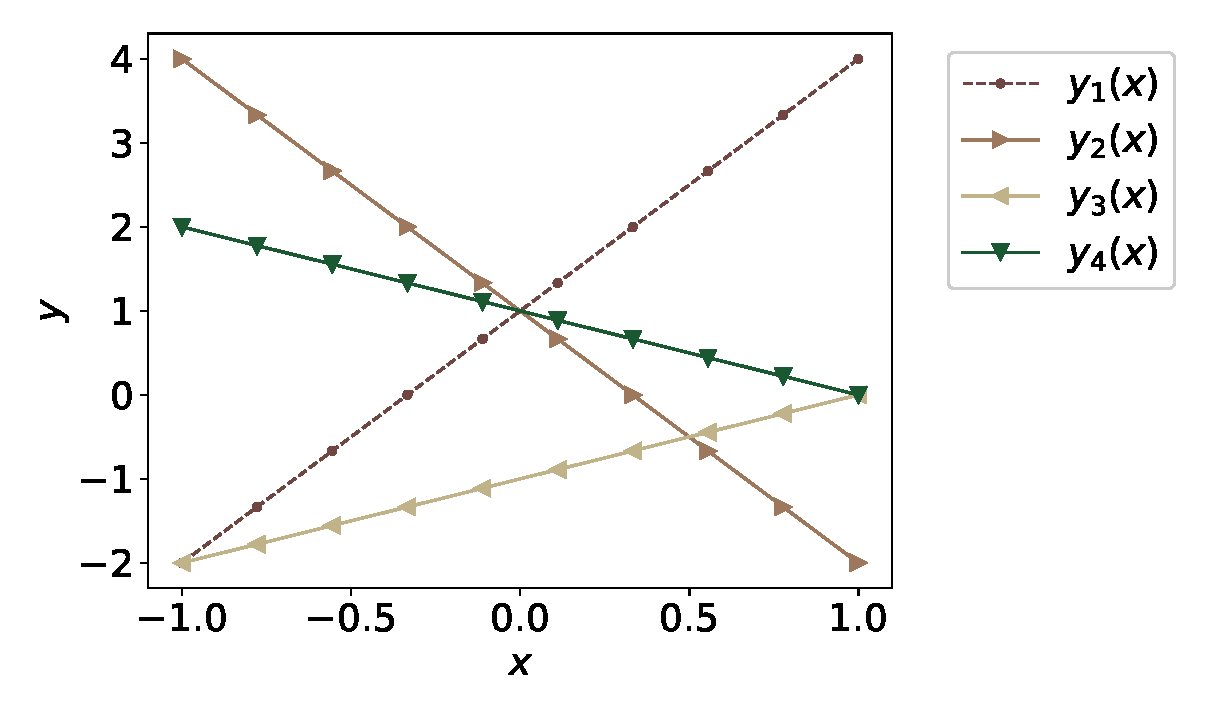
\includegraphics[width=0.75\textwidth]{chapters/cap1/python/example.eps}
  \caption{Image with the same color scheme of book} % Adiciona uma legenda
  \label{fig:exemplo} % Adiciona um rótulo para referência
\end{figure}


\begin{theorem}[Name of the theorem]
\label{theo:ex1:A}
\lipsum[1][1-3]
\begin{equation}
x^2+e^{-\frac{x^2}{2}}=1
\end{equation}
\end{theorem}

teste

\begin{proofraw}[Relative to Teorema \ref{theo:ex1:A}]
\lipsum[1][1-3]
\begin{equation}
x^2+e^{-\frac{x^2}{2}}=1
\end{equation}
\end{proofraw}
%-------------------------------------------------------------------------------
\section{Lists}\index{Lists}

\lipsum[1][1-3]\footnote{Footnote example...}.

\subsection{Numbered List}\index{Lists!Numbered List}

\begin{enumerate}
\item \lipsum[1][1-3].
\item \lipsum[1][1-3].
\item \lipsum[1][1-3].
\end{enumerate}

\subsection{Bullet Points}\index{Lists!Bullet Points}

\begin{itemize}
\item \lipsum[1][1-3].
\item \lipsum[1][1-3].
\item \lipsum[1][1-3].
\end{itemize}

\subsection{Descriptions and Definitions}\index{Lists!Descriptions and Definitions}

\begin{description}
\item[Name] \lipsum[1][1-3].
\item[Word] \lipsum[1][1-3].
\item[Comment] \lipsum[1][1-3].
\end{description}

